%!TEX root = ../memoria.tex

\chapter{Otros Formatos UTFSM para Memorias y Tesis de Grado [Obsoleto]}

\section{Otros Formatos UTFSM [OBSOLETO]}

Todo archivo para titulación actualmente se maneja exclusivamente en formato digital.

Las siguientes secciones se mantienen sólo para fines de legado y registro histórico.

\subsection{Formato de las Cubiertas (Empaste)}

A partir del año 2016, ya no es necesaria la entrega de una copia física de la memoria o tesis, siendo esto opcional. Si decide imprimirla, estás son las normas para el empaste.

La cubierta o tapa será de empaste duro, cubierta de vinilo o similar de color NEGRO con letras doradas, según se muestran en \autoref{fig:thesis_cover} y \autoref{fig:thesis_cover_lateral}.

\begin{figure}[ht!]
\centering
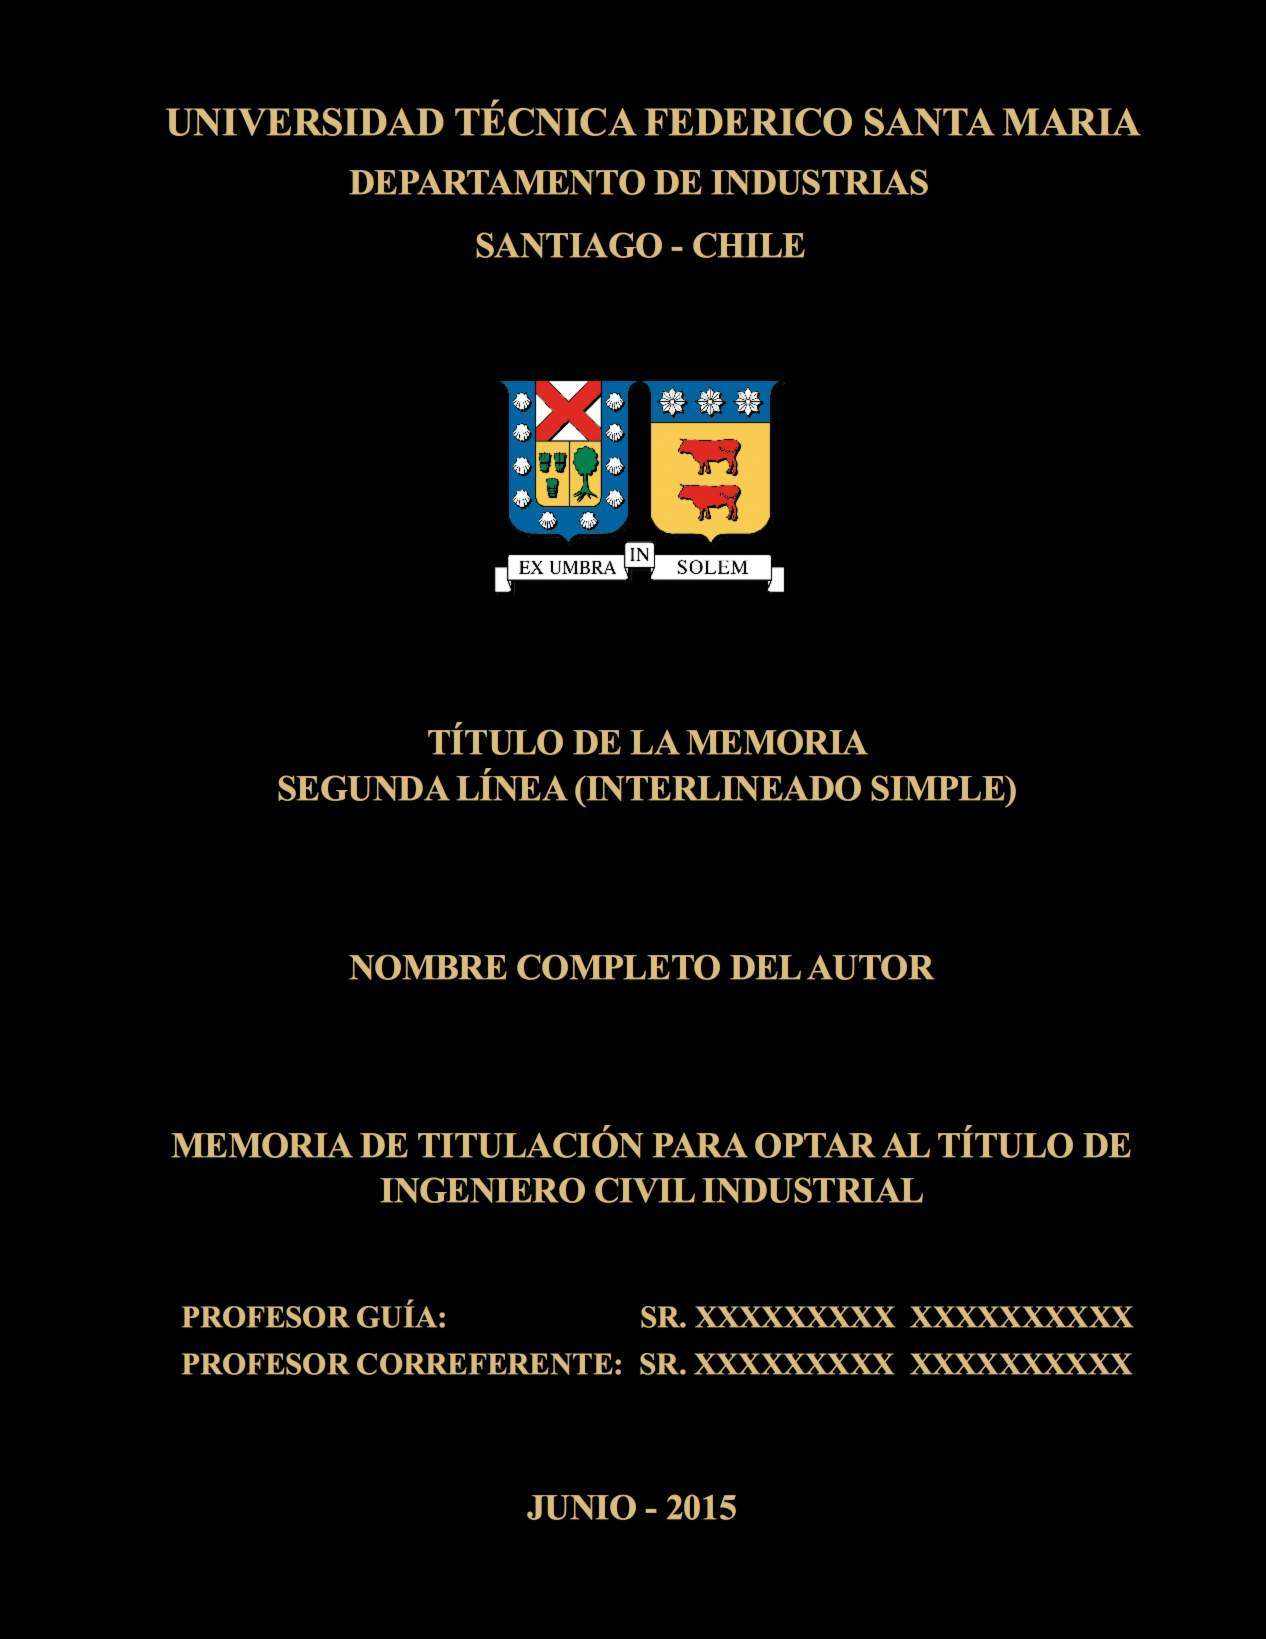
\includegraphics[width=.7\textwidth]{figures/thesis_cover.png}
\caption{Cubierta (Empaste) Memorias y Tesis UTFSM.}
\label{fig:thesis_cover}
\end{figure}

\begin{figure}[ht!]
\centering
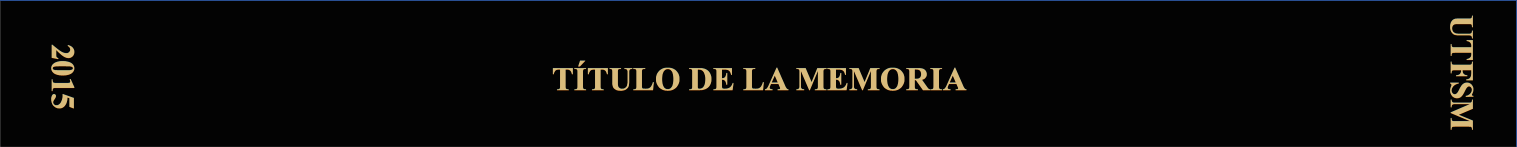
\includegraphics[width=.7\textwidth]{figures/thesis_cover_lateral.png}
\caption{Lomo del Empaste para Memorias y Tesis UTFSM.}
\label{fig:thesis_cover_lateral}
\end{figure}

\subsection{Formato del Disco Compacto}

El CD/DVD debe tener una carátula de identificación circular con fondo blanco, conteniendo las siguientes leyendas:

\begin{itemize}
		\item
    Centrado en la parte superior: UTFSM, con letras mayúsculas en negrita tamaño 12. A renglón seguido el nombre de la Unidad Académica con letras mayúsculas en negrita tamaño 10.
		\item
    Centrado en la parte inferior el nombre completo del alumno con letras mayúsculas en negrita tamaño 10.
		\item
    Tres espacios más abajo y centrado, “TÍTULO DE LA MEMORIA”, con letras mayúsculas en negrita tamaño 10.
		\item
    Dos espacios más abajo y centrado MES –AÑO, con letras mayúsculas en negrita tamaño 10.
    En el lado izquierdo y centrado, el escudo en colores de la Institución.
		\item
    En el lado derecho y centrado, NOMBRE DE LA UNIDAD ACADÉMICA y la ubicación CIUDAD – PAIS, con letras mayúsculas en negrita tamaño 8.
\end{itemize}

\begin{figure}[ht!]
\centering
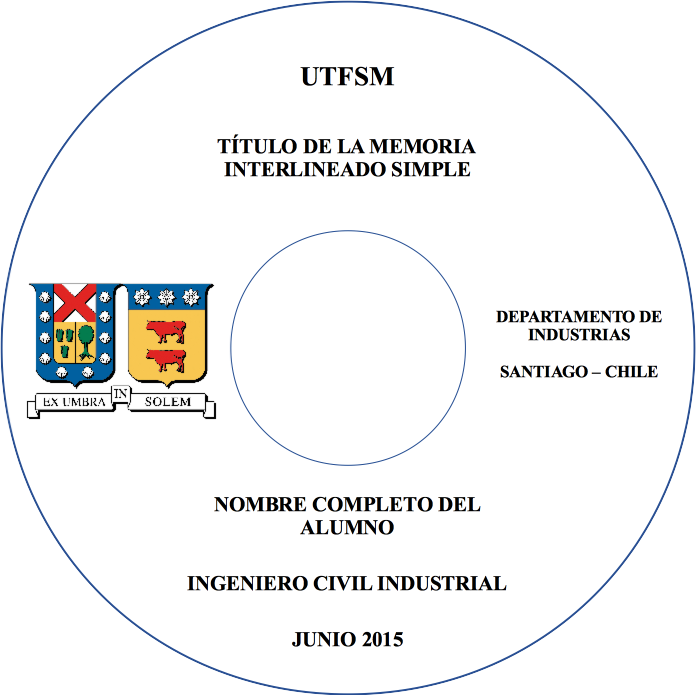
\includegraphics[width=.4\textwidth]{figures/thesis_cd.png}
\caption{Disco Compacto para Memoria UTFSM}
\label{fig:thesis_cd}
\end{figure}


Los CD se guardarán, en la biblioteca, en una caja de acrílico que tendrá una carátula de identificación dividida en tres franjas iguales, con las siguientes leyendas:
\begin{itemize}
		\item
    El escudo a color de la Institución de 20 mm de alto, centrado en la franja superior.
		\item
    El nombre completo del alumno, y centrado dos espacios más abajo el título de la memoria, en la franja del medio
		\item
    El nombre de la Unidad Académica, y renglón más abajo, año. En la franja inferior.
\end{itemize}


\begin{figure}[ht!]
    \centering
    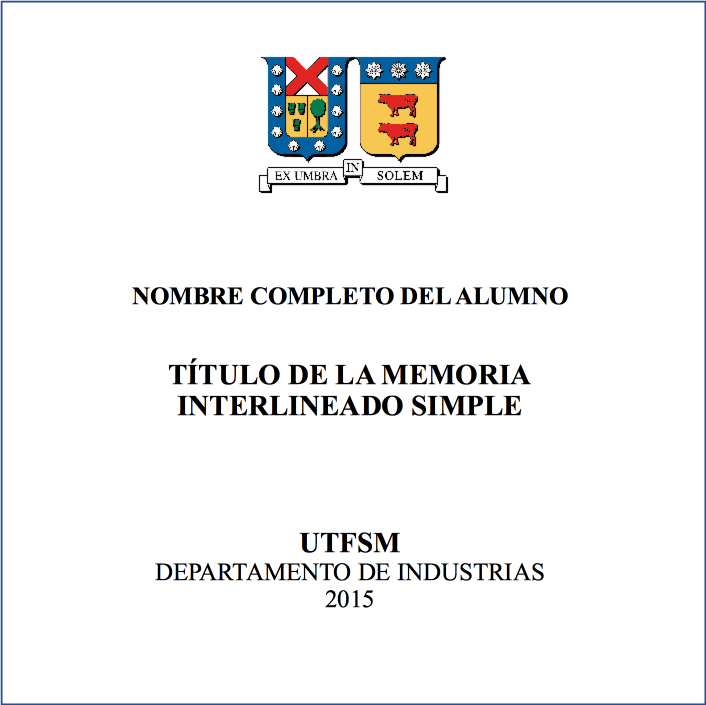
\includegraphics[width=.4\textwidth]{figures/thesis_cd_cover.png}
    \caption{Cubierta de Disco Compacto para Memorias y Tesis UTFSM.}
    \label{fig:thesis_cd_cover}
\end{figure}


